\section{Reference-Compatible Execution}
\label{sec:method}
\subsection{Derive query groups from live cache geometry}
A backend recipe specifies the reference-compatible activation and weight types, reduction organization, placement, supported shapes and strides, and output layout. Source analysis, own-path replay and cross-path comparisons on captured model operands establish this recipe offline. At runtime, descriptor guards select it from the current phase and operator metadata. The planner then groups queries whose live geometry allows them to share that recipe.

For the supported dense, nonwrapping append profile, the extractor reads occupancy, physical head, capacity and padding. It checks that occupied cells form the logical prefix and that the head agrees with its end. If $H$ is the first appended physical slot, $i$ is the zero-based query-row index, $N$ is capacity and $P$ is padding, the required extent is
\begin{equation}
 e_i=\min\!\left(N,\max\!\left(P,P\left\lceil\frac{H+i+1}{P}\right\rceil\right)\right).
 \label{eq:extent}
\end{equation}
Each query carries its logical position, $e_i$, arithmetic class and original requested-output flag. The plan is determined from these descriptors before executing the call.

Adjacent queries with the same extent and arithmetic class form maximal compatible runs. Each native call supports at most $W_{\max}$ rows. For run lengths $r_1,\ldots,r_m$, the minimum number of contiguous calls under these constraints is
\begin{equation}
 G_{\min}=\sum_{j=1}^{m}\left\lceil r_j/W_{\max}\right\rceil.
 \label{eq:groups}
\end{equation}
A key change forces a cut; otherwise the next call takes the longest supported prefix. This produces the $3+1$ split for positions 765--768. The same rule produces a $1+3$ split from physical head 767, where the extents are $[768,1024,1024,1024]$. Both splits follow from current cache metadata.

The grouping pass is linear in the number of queries; the dense-cache validator additionally scans the occupied prefix. Graph-reuse keys include the recipe, per-row geometry and phase policy alongside the outer shape. Validation, planning and reuse checks remain part of the executed service.

\subsection{Choose where to place the cuts}
Whole-graph execution (W) runs projection, attention and feed-forward computation for each compatible query group. It restarts maximal grouping after a physical boundary, combining all adjacent rows allowed by the current requirements and width bound. This provides a simple compatible path and the baseline for evaluating local cuts.

Local execution (L) keeps the outer graph wide and places the cuts inside attention. Q, K, V and mask views select each group's required range. The adapter provides the strides and contiguous materialization required by the native attention recipe, then restores attention outputs to logical query order. Projection and feed-forward work outside attention can consequently process more rows together. The physical groups retain their required execution order; the wider outer work is available because the input query rows are already known.

Cut placement and projection arithmetic are independent choices (Fig.~\ref{fig:execution_method}): changing where attention is split need not change how a projection reduces its operands.

\begin{figure*}[t]
\centering
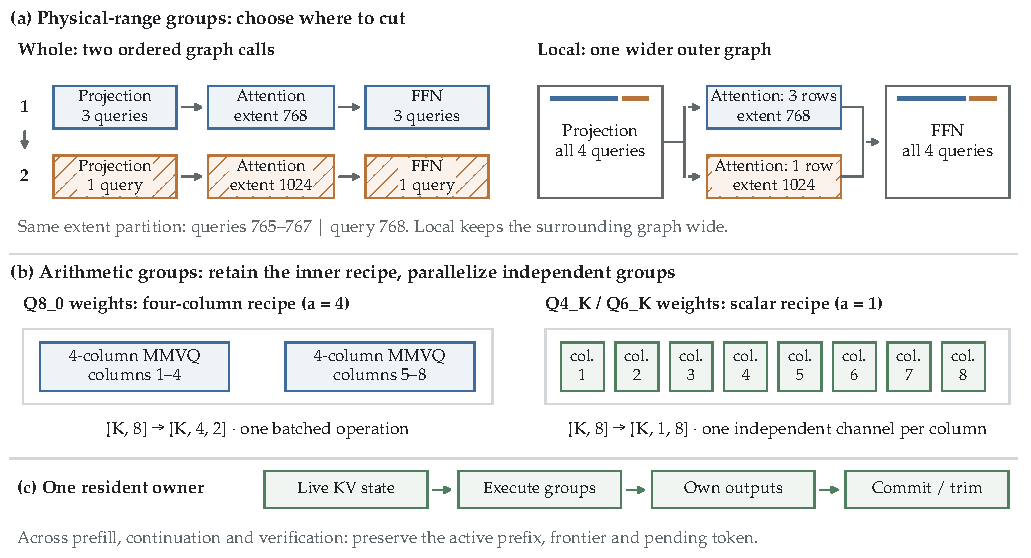
\includegraphics[width=\textwidth]{figures/execution_method.pdf}
\caption{Two choices in reference-compatible execution. Whole execution splits the complete graph into compatible query groups; Local execution confines these cuts to attention and retains wider outer work. The projection, attention and feed-forward blocks repeat across transformer layers. Separately, GPU packing exposes independent arithmetic groups while preserving their inner computation: four columns for the affected CUDA Q8 path and one column for the mixed Q4\_K/Q6\_K path. Physical-extent groups and arithmetic groups serve different constraints. Requested outputs and commit/trim operations share one resident target/KV owner.}
\label{fig:execution_method}
\end{figure*}

\subsection{Expose independent arithmetic groups to the GPU}
\label{sec:recipes}
A wider projection is useful only if its inner computation remains compatible. Let $X\in\mathbb{R}^{K\times q}$ contain $q$ query columns and let $a$ be the native arithmetic group width selected by the recipe. For $q=ag$, a view exposes the independent group index:
\begin{equation}
 \widetilde X_{k,c,j}=X_{k,aj+c},\quad
 \widetilde X\in\mathbb{R}^{K\times a\times g}.
 \label{eq:packing}
\end{equation}
The backend broadcasts the shared weights across $g$ groups and retains the computation within each group. A final view restores logical column order. Eligible shapes and layouts are checked before this mapping; tails use their validated native path.

\subsubsection{CUDA Q8}
For the affected Q8\_0 projections with F32 input, $a=4$ retains the small-column MMVQ computation identified in Section~\ref{sec:reference}. The backend-loop4 control quantizes the input and invokes that specialization for successive groups and the supported tail. Packing uses $[K,4,g]$ views to replace successive backend invocations with one grouped operation. The GPU executes the groups independently while each retains the four-column reduction organization.

A $k=3$ speculative transaction requests at most four target positions, so its verification does not enter the multi-group packing route. Wider prompt work can still use packing. A $k=7$ transaction can request eight positions and expose two groups. Draft prefill width is an independent application parameter.

\subsubsection{Mixed Q4\_K/Q6\_K}
The 32B extension preserves scalar-column computation for the affected Q4\_K and Q6\_K projections, giving $a=1$. Its graph-level control creates scalar-column views, matrix operations and concatenations. Grouping maps the same columns to $[K,1,q]$ and executes them as independent channels. The original per-type dot functions, activation quantizer and accumulation organization are retained. This extends the typed recipe while leaving the Q8 four-column rule intact. Full-model service comparisons use the graph-level scalar-column control; native-operator controls additionally examine the cost of its implementation.

\subsubsection{Vulkan}
The Vulkan mapping retains F32 activations for the affected Q8 projections and dispatches independent column tiles across the GPU grid. In attention, the p021 QK specialization is extended across query workgroups to retain its scalar reduction; AV uses each group's required physical range and qualified stride/dispatch. Recipe selection is phase-specific: the original prompt producer retains its arithmetic, while continuation and verification use the corresponding projection and attention paths. The same physical-prefix planning interface supports two-query verification and wider known-query append, with backend-specific arithmetic beneath it.

\subsection{Carry logical outputs and state across phases}
Prefill, ordinary continuation and verification operate on one resident target/KV owner. A phase transition selects the appropriate recipe and plan while retaining this state. Output reservation specifies storage capacity; the original requested-row mask determines which vectors the call must produce. Table~\ref{alg:plan} summarizes the phase execution.

After each native call, the executor synchronizes and copies its requested vectors into logical output slots before later calls can reuse the scratch buffer. A commit can then select the frontier of the accepted prefix even when a later physical row was rejected. Trimming updates active KV and the logical frontier together. The pending-token record preserves an emitted correction or bonus token until the next phase materializes it, including native cap and end-of-generation behavior. Reset restores the declared initial state; a failed native call invalidates the partially updated owner.

\begin{table}[t]
\centering\footnotesize
\caption{Execution of one reference-derived phase.}
\label{alg:plan}
\begin{minipage}{\columnwidth}
\textbf{Input:} resident state $S$, phase $p$, known rows $Q$ and original requested-row mask $O$.
\begin{enumerate}[leftmargin=1.6em,itemsep=2pt,topsep=4pt]
\item Select the arithmetic recipe from phase and operator descriptors.
\item Check capacity, cache ownership and recipe support; extract each row's physical extent.
\item Form adjacent compatible groups and place whole-graph or attention-local cuts.
\item Apply the supported arithmetic-group packing.
\item Execute native calls in logical order with the original output requests; own requested vectors before scratch reuse.
\item Commit or trim using the owned frontier and pending-token record.
\item Retain the updated owner on success; invalidate it after a failed native call.
\end{enumerate}
\end{minipage}
\end{table}

The argument for Eq.~\eqref{eq:contract} starts from state that matches the reference after the same logical phase history. The recipe must preserve the required outputs and state update for each native group; output ownership and commit/trim must retain the corresponding logical state for the next phase. Under these conditions, induction over groups and phase boundaries preserves the reference relation. Native replays and full-model state checks test these premises in the implemented deployments. Qualification uses independent-reference replay and heavy state capture; service measurements include planning, synchronization, output copies and state updates.
